\documentclass[]{article}
\usepackage{graphicx}

\begin{document}
\begin{titlepage}
\begin{center}
	\includegraphics[scale=0.25]{/home/dieguito/Pictures/logo_udeg_negro.png}\\
	\vspace{1cm}
{\Large 	\textbf{Centro Universitario de Ciencias Exactas e Ingenierías}\\}

\vspace{0.5cm}
	
{\large 	\textit{Departamento de ciencias computacionales}\\}
	
	\vspace{1cm}
	
	\textbf{Administración de redes}\\
	
	\vspace{0.5cm}
	
	\textbf{Reporte semanal}\\
	
	\vspace{0.5cm}
	
	Semana \textbf{4}
	
	\vspace{0.5cm}
	
	\underline{Título del reporte}\\
	
	\vspace{1cm}
	
	Prof: Ing. Luis Ignacio Sánchez Salazar\\
	
	Alumno: Diego Martín Domínguez Hernández\\
	
	Carrera: Ingeniería Informática \\
	
	Materia: i5907 (Administración de Redes)\\
	
	NRC: 42241\\
	
	Sección: D04\\

	Calendario: 2023A\\
	
\end{center}
\end{titlepage}
	\begin{center}
		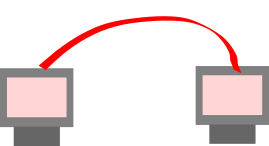
\includegraphics[scale=0.25]{computadoras.png}
	\end{center}
\begin{enumerate}
	\item Revisar configuración de red de las
		computadoras que intervienen en el
		proceso
	\begin{enumerate}
		\item Modelo y marca de la tarjeta
			de red
		\item Tomar imagen Ipv4 (para
			regresarlos al final)
	\end{enumerate}
	\item Cambiar IPv4
	\begin{enumerate}
		\item 192.168.1.1/24
		\item 192.168.1.2/24
	\end{enumerate}
	\item Generar una cuenta usuario
		"sin privilegios"
	\item Debajo de \textit{C:users}
		crear carpeta \textit{comparteRedes}
	\item Compartir la carpeta con el usuario
		que pueda escribir
	\item Transferir entre las computadoras
		A y B archivos de 50MB
		y tomar los siguientes tiempos:
	\begin{itemize}
		\item 10Mb Half-Duplex
		\item 10Mb Full-Duplex
		\item 100Mb Full-Duplex
	\end{itemize}
\end{enumerate}
\end{document}
